% Created 2024-04-14 Sun 19:04
% Intended LaTeX compiler: pdflatex
\documentclass[10pt,table,dvipsnames,compress]{beamer}
\usepackage[utf8]{inputenc}
\usepackage[T1]{fontenc}
\usepackage{graphicx}
\usepackage{longtable}
\usepackage{wrapfig}
\usepackage{rotating}
\usepackage[normalem]{ulem}
\usepackage{amsmath}
\usepackage{amssymb}
\usepackage{capt-of}
\usepackage{hyperref}
\usetheme{default}
\useinnertheme{rounded}
\useoutertheme[subsection=false]{miniframes}
\date{}
\title{MELANOBS: forest cover change, carbon, and biodiversity data in Melanesia}
\title[MELANOBS]{MELANOBS: forest cover change, carbon, and biodiversity data in Melanesia}
\usepackage{lmodern}
\usepackage{pgf}
\usepackage{color}
\usepackage[english,french]{babel}
\definecolor{vertmoyen}{RGB}{51,110,23} % vert moyen
\definecolor{blueFRB}{HTML}{31859c}
\usecolortheme[named=blueFRB]{structure}
\usepackage{tabularx} % varier la largeur du tableau
\usepackage{layout}
\setlength{\LTleft}{-5cm plus 1 fill}
\setlength{\LTright}{-5cm plus 1 fill}
\usepackage{booktabs}
\usepackage{arydshln} %% dashlines for tabular
\newcommand{\logit}{\text{logit}}
\newcommand{\bs}[1]{\boldsymbol{#1}}
\newcommand{\R}{\textnormal{\sffamily\bfseries R}}
\newcommand{\pkg}[1]{{\fontseries{b}\selectfont #1}}
\newcolumntype{C}[1]{>{\centering\arraybackslash}m{#1}}

\setbeamertemplate{footline}[frame number]
\setbeamertemplate{frametitle}{%
\usebeamerfont{frametitle}\insertframetitle%
\vphantom{g} % To avoid fluctuations per frame
\par
\centering 
\includegraphics[width=\textwidth]{figs/Barre_couleur}
}
\beamertemplatenavigationsymbolsempty

% Logo
\newif\ifplacelogo % create a new conditional
\logo{\ifplacelogo
\includegraphics[width=0.5\textwidth]{figs/partners_logos}\fi}

%Call table of contents at the beginning of each section
\AtBeginSection[]{
\placelogotrue
\begin{frame}
\frametitle{Plan}
\begin{columns}[c]
\begin{column}{0.5\textwidth}
\tableofcontents[sections=1,currentsection]
\vspace{0.5cm}
\tableofcontents[sections=2,currentsection]
\vspace{0.5cm}
\tableofcontents[sections=3,currentsection]
\end{column}
\begin{column}{0.5\textwidth}
\tableofcontents[sections=4,currentsection]
\vspace{0.5cm}
\tableofcontents[sections=5,currentsection]
\end{column}
\end{columns}
\end{frame}
\placelogofalse
}

\AtBeginSubsection[]{}

\hypersetup{
colorlinks=true,
linkcolor=Black,
filecolor=Maroon,
citecolor=Blue,
urlcolor=Maroon}

% Disable monospaced font for URLs
\urlstyle{same}

\hypersetup{
 pdfauthor={Ghislain Vieilledent},
 pdftitle={MELANOBS: forest cover change, carbon, and biodiversity data in Melanesia},
 pdfkeywords={},
 pdfsubject={},
 pdfcreator={Emacs 29.2 (Org mode 9.6.15)}, 
 pdflang={English}}
\begin{document}


% {
%   % Use background image
%   \usebackgroundtemplate{%
%     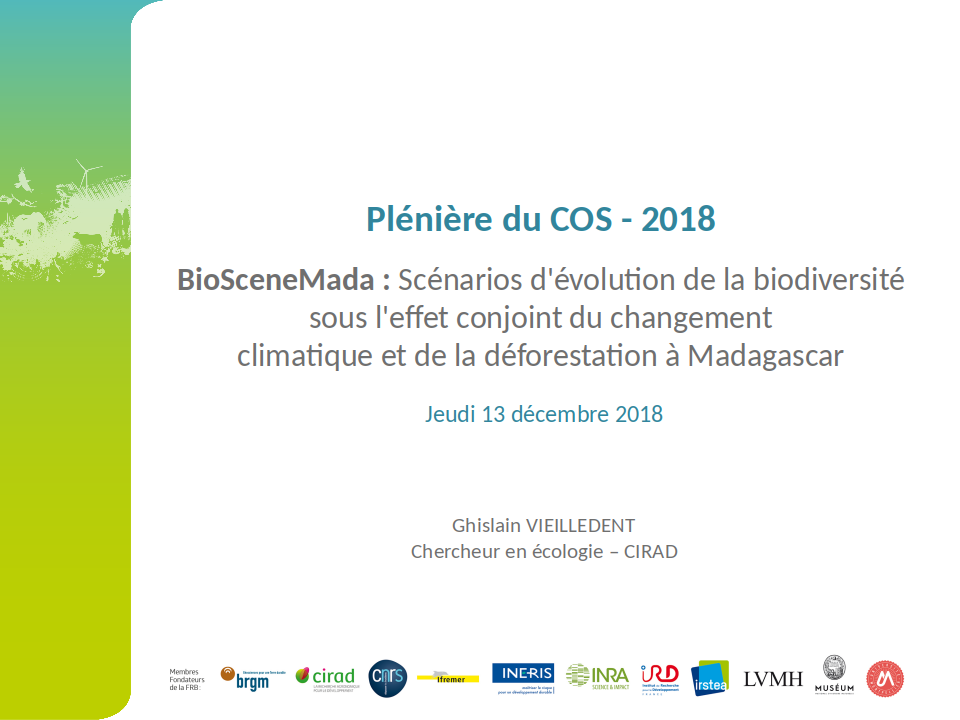
\includegraphics[height=\paperheight,width=\paperwidth]{figs/Masque.png}
%   }
%   \setbeamertemplate{navigation symbols}{}
%   % Remove shadow from block
%   \setbeamertemplate{blocks}[rounded][shadow=false]
%   \begin{frame}[plain]
%   \end{frame}
% }

% Title page
{
  \setbeamertemplate{navigation symbols}{}
  \begin{frame}[plain, noframenumbering]
  \begin{center}
  \small{\textbf{MELANOBS workshop -- Noumea, April 2024}}
  \end{center}
  \vspace{-0.5cm}
  \titlepage % Presentation first page
  \vspace{-3cm}
  \begin{center}
    
\includegraphics[width=\textwidth]{figs/Barre_couleur}
    
    \vspace{0.25cm}
    
    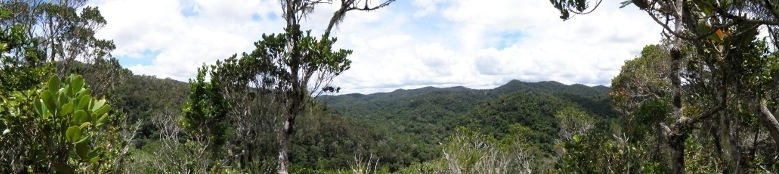
\includegraphics[width=10cm]{figs/Banniere}
    
    \small{Ghislain VIEILLEDENT$^{1}$\hspace{0.25cm}Philippe BIRNBAUM$^{1}$\\
      \vspace{0.10cm}David BRUY$^{2}$\hspace{0.25cm}Thomas IBANEZ$^{2}$}
      
    \vspace{0.25cm}
    
    {\scriptsize
      \begin{tabular}{l}
        $[1]$ \textbf{Cirad} UMR AMAP, $[2]$ \textbf{IRD} UMR AMAP
      \end{tabular}
    }
    
    
\includegraphics[width=0.6\textwidth]{figs/partners_logos}
    
  \end{center}
  \end{frame}
}

% %%%%%%%%%%%%%%%%%%%%%%%%%%%%%%%%%%%%%%%%%%%%%%%%%%%%%%%%%%%%%%%%

\placelogotrue
\begin{frame}
  \frametitle{Outline}
  \begin{columns}[c]
    \begin{column}{0.5\textwidth}
      \tableofcontents[sections=1]
      \vspace{0.5cm}
      \tableofcontents[sections=2]
      \vspace{0.5cm}
      \tableofcontents[sections=3]
    \end{column}
    \begin{column}{0.5\textwidth}
        \tableofcontents[sections=4]
        \vspace{0.5cm}
        \tableofcontents[sections=5]
    \end{column}
  \end{columns}
\end{frame}
\placelogofalse

\section{Introduction}
\label{sec:org623e54e}

\subsection{Context}
\label{sec:orgf754b91}

\begin{frame}[label={sec:org1754275}]{Context}
\begin{center}
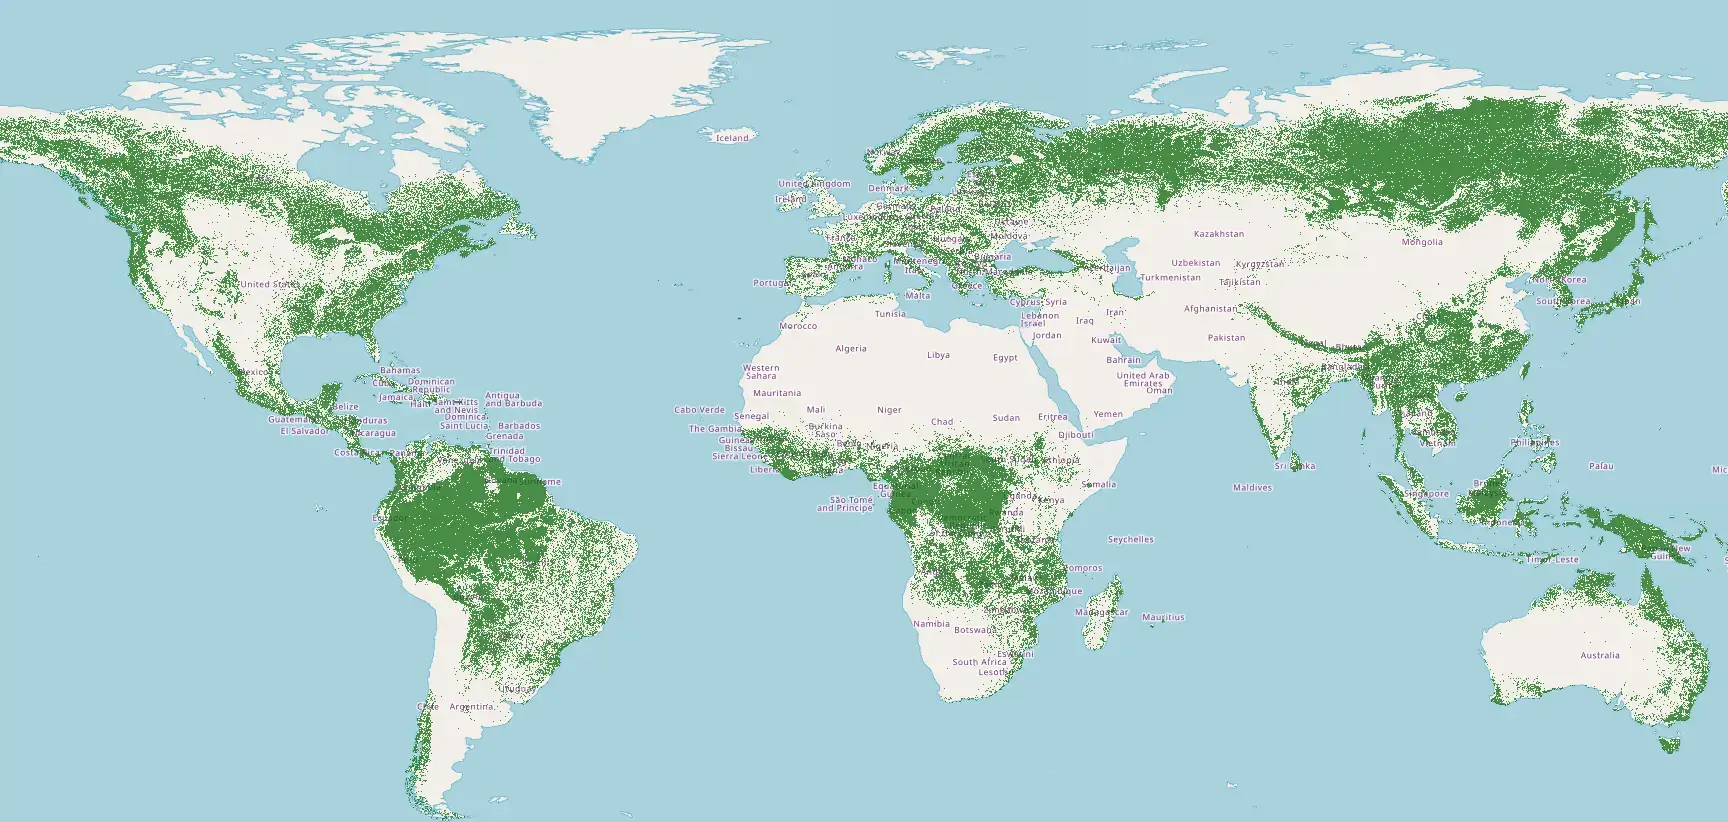
\includegraphics[width=8cm]{figs/forest_cover_jrc_2020.png}
\end{center}

\begin{itemize}
\item Tropical forests: 50\% of terrestrial biodiversity.
\item Tropical deforestation: 15\% of anthropogenic carbon emissions.
\item Mapping forest cover, carbon stocks and biodiversity is essential for conservation planning.
\end{itemize}
\end{frame}

\subsection{Objectives}
\label{sec:org6327cca}

\begin{frame}[label={sec:orgd56687c}]{Objectives}
\begin{center}
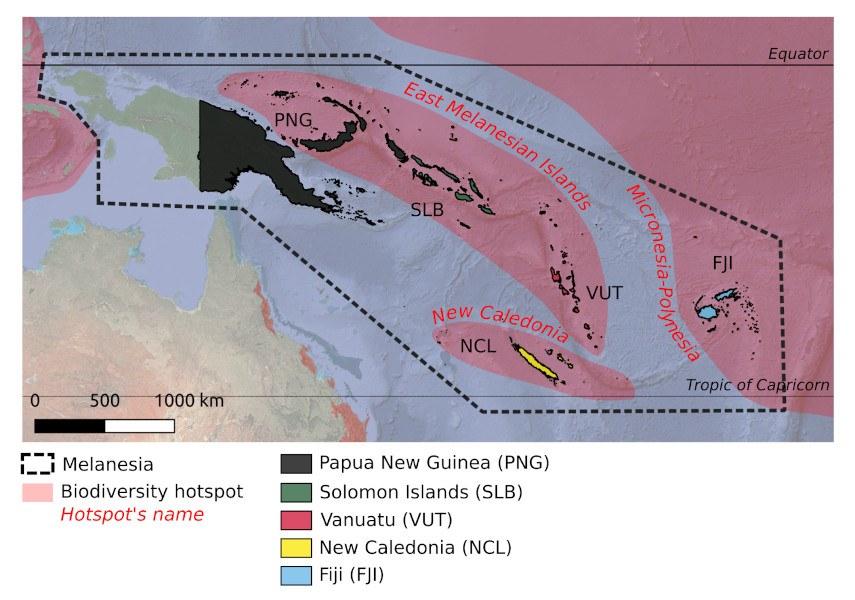
\includegraphics[width=8cm]{figs/carte_melanobs.jpg}
\end{center}

\begin{itemize}
\item MELANOBS: building a Melanesian forest observatory.
\item Which data on forest cover, carbon stock and biodiversity are available for Melanesian countries?
\end{itemize}
\end{frame}

\section{Forest cover change maps}
\label{sec:orgfe3340d}

\subsection{FAO FRA estimates}
\label{sec:org0189183}

\begin{frame}[label={sec:orgb02b39d}]{FAO FRA estimates, forest cover}
\textbf{Forest cover estimates (in Kha).}

\begin{center}
\footnotesize
\begin{tabular}{lrrrr}
Country & FRA 2015 & prim. forest & GFC30 2020 & TMF 2020\\[0pt]
\hline
PNG & 36024 & 27200 & 39000 & 39304\\[0pt]
Solomon Islands & 2527 & 1738 & 2350 & 2739\\[0pt]
Vanuatu & 442 & 205 & 986 & 1152\\[0pt]
Fiji & 1107 & 0 & 1050 & NA\\[0pt]
New Caledonia & 839 & 338 & 1150 & 855\\[0pt]
\end{tabular}
\end{center}

\begin{itemize}
\item Forest Ressources Assessment (FRA) from the Food and Agriculture Organization (FAO).
\item Estimates are reported by countries to FAO.
\item Differentiate forest types: forest, primary forest, plantations
\item Not frequently updated.
\item Information is not spatialized.
\end{itemize}
\end{frame}

\begin{frame}[label={sec:org0a93774}]{FAO FRA estimates, forest cover}
\textbf{Forest cover estimates (in \% of land area).}

\begin{center}
\footnotesize
\begin{tabular}{lrlll}
Country & Area (km2) & FRA 2015 & GFC30 2020 & TMF 2020\\[0pt]
\hline
PNG & 462840 & 78\% & 84\% & 85\%\\[0pt]
Solomon Islands & 28896 & 87\% & 81\% & 95\%\\[0pt]
Vanuatu & 12189 & 36\% & 81\% & 95\%\\[0pt]
Fiji & 18272 & 61\% & 57\% & NA\\[0pt]
New Caledonia & 18575 & 45\% & 62\% & 46\%\\[0pt]
\end{tabular}
\end{center}

\begin{itemize}
\item Forest Ressources Assessment (FRA) from the Food and Agriculture Organization (FAO).
\item Estimates are reported by countries to FAO.
\item Differentiate forest types: forest, primary forest, plantations.
\item Not frequently updated.
\item Information is not spatialized.
\end{itemize}
\end{frame}

\begin{frame}[label={sec:org5e040cc}]{FAO FRA estimates, deforestation}
\textbf{Mean annual deforestation (in ha).}

\begin{center}
\footnotesize
\begin{tabular}{lrrr}
Country & FRA & GFC30 & TMF\\[0pt]
 & 2015--2020 & 2010--2020 & 2010--2020\\[0pt]
\hline
PNG & 34000 & 104678 & 48691\\[0pt]
Solomon Islands &  & 13460 & 1751\\[0pt]
Vanuatu &  & 939 & 564\\[0pt]
Fiji &  & 2663 & \\[0pt]
New Caledonia &  & 1328 & 2425\\[0pt]
\end{tabular}
\end{center}

\begin{itemize}
\item Rather good estimates of forest cover but poor estimates of deforestation/regrowth.
\end{itemize}
\end{frame}

\begin{frame}[label={sec:org952a15d}]{FAO FRA estimates, deforestation}
\textbf{Mean annual deforestation (in \%/yr).}

\begin{center}
\footnotesize
\begin{tabular}{lrrr}
Country & FRA & GFC30 & TMF\\[0pt]
 & 2015--2020 & 2010--2020 & 2010--2020\\[0pt]
\hline
PNG & 0.09 & 0.27 & 0.12\\[0pt]
Solomon Islands &  & 0.57 & 0.06\\[0pt]
Vanuatu &  & 0.1 & 0.05\\[0pt]
Fiji &  & 0.25 & \\[0pt]
New Caledonia &  & 0.12 & 0.28\\[0pt]
\end{tabular}
\end{center}

\begin{itemize}
\item Rather good estimates of forest cover but poor estimates of deforestation/regrowth.
\end{itemize}
\end{frame}

\subsection{Global maps}
\label{sec:orga51ffc0}

\begin{frame}[label={sec:orge595ab1}]{Global Forest Change (GFC)}
\begin{center}
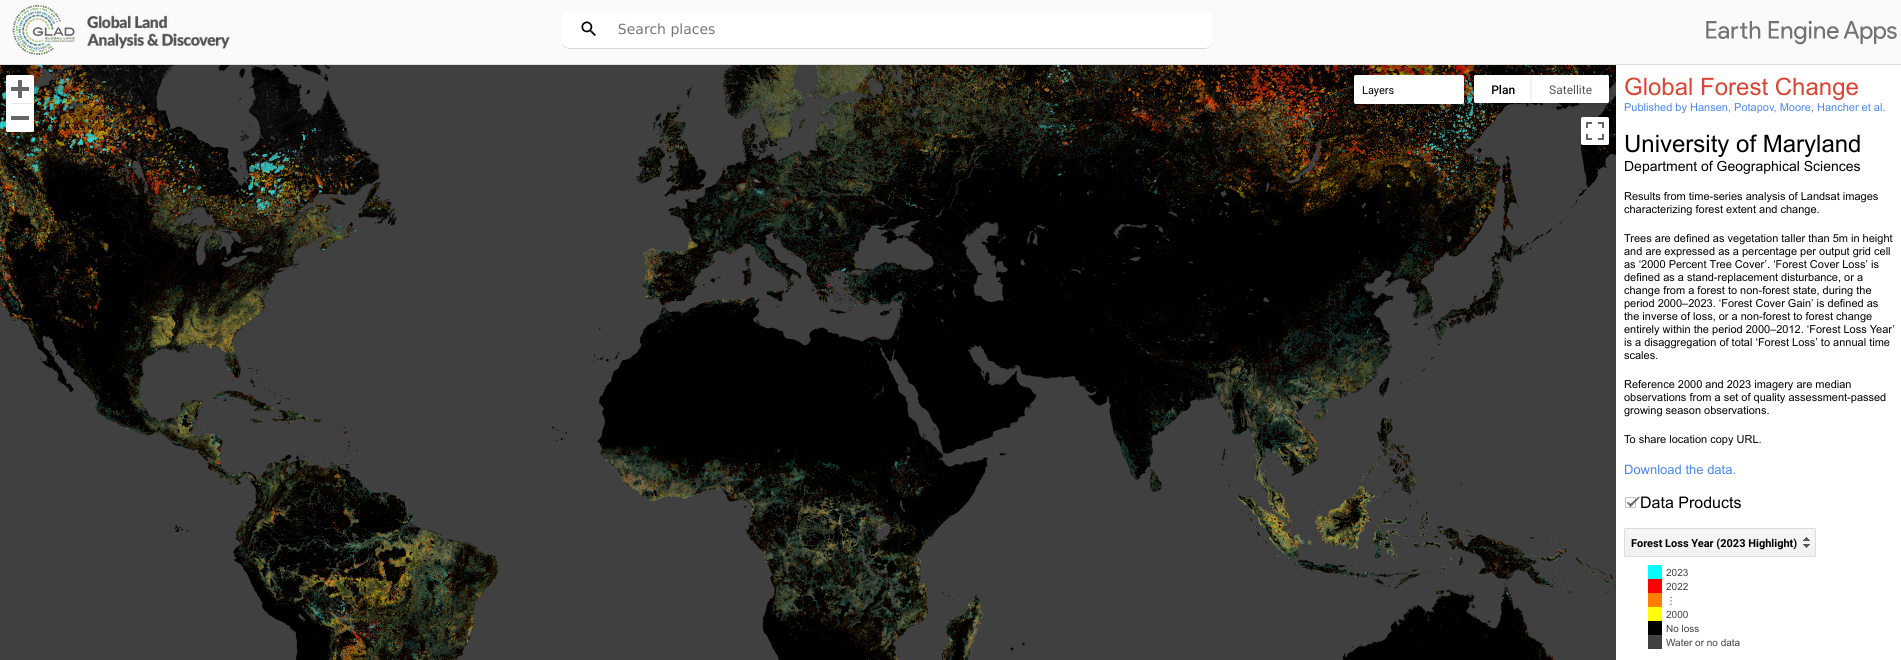
\includegraphics[width=8cm]{figs/fcc/gfc.png}
\end{center}

\begin{itemize}
\item \href{https://glad.earthengine.app/view/global-forest-change}{Global Forest Change} (Hansen et al. 2013, Univ. of Maryland).
\item Used by \href{https://www.globalforestwatch.org/}{Global Forest Watch} (GFW): platform about the world forests. GFW releases the \href{https://research.wri.org/gfr/global-forest-review}{Global Forest Review}.
\item It is in fact a tree cover change product. User must define a tree cover threshold to define the forest (e.g. 30\%).
\item Derive from Landsat images from 2000. 30m resolution. One mosaic per year.
\item Largely overestimate forest cover if low tree cover threshold (e.g. 30\%).
\item Underestimate small-scale deforestation (shifting agriculture, logging).
\end{itemize}
\end{frame}

\begin{frame}[label={sec:org2d4c8f6}]{Tropical Moist Forests (TMF)}
\begin{center}
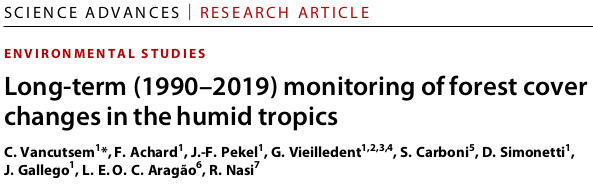
\includegraphics[width=8cm]{figs/fcc/Vancutsem2021.png}
\end{center}

\begin{itemize}
\item \href{https://forobs.jrc.ec.europa.eu/TMF}{Tropical Moist Forests} (Vancutsem et al. 2021, from Joint Research Center).
\item Only consider evergreen tropical forests (tropical moist forests, mangroves, evergreen dry tropical forests). Cannot be used to monitor deciduous dry forests.
\item Derive from Landsat images from 1990. 30m resolution. Time-series at the pixel scale.
\item Fiji is not entirely available (beyond the 180th meridian).
\item Overestimate forest cover in some areas (e.g. Vanuatu, Mare island in New Caledonia).
\end{itemize}
\end{frame}

\subsection{National data}
\label{sec:org6fd29ef}

\begin{frame}[label={sec:org53ea6db}]{National data}
\begin{itemize}
\item There is room to improve forest cover change maps at the national scale.

\item MELANOBS objectives:
\begin{itemize}
\item Which forest cover change data is available at the national scale?
\item Derive up to date forest cover change maps for participating countries.
\end{itemize}
\end{itemize}
\end{frame}

\begin{frame}[label={sec:org31706ad}]{In New-Caledonia}
\begin{center}
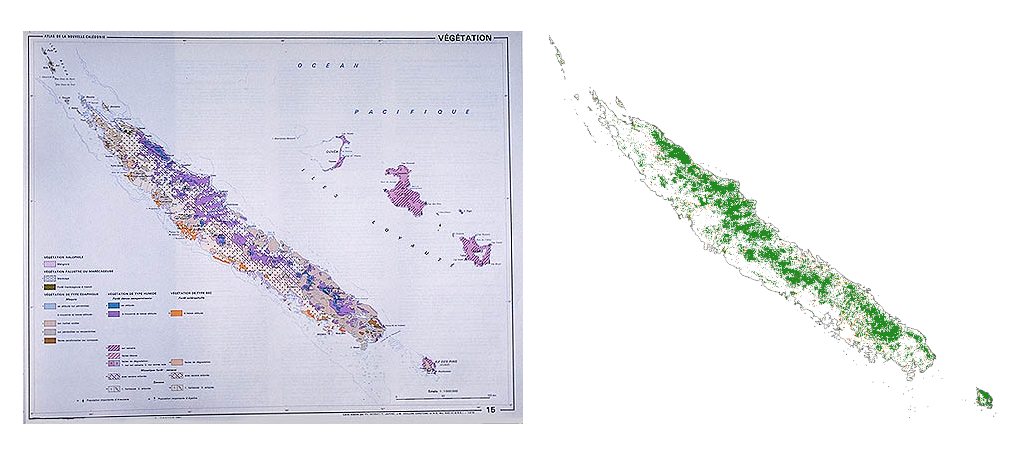
\includegraphics[width=9cm]{figs/fcc/fcc_nc.png}
\end{center}

\begin{itemize}
\item Coarse vegetation maps from IRD (Jaffre, Morat).
\item Forest cover change map for 2000-2010-2020 derived from TMF.
\item Natural forest cover map for year \textasciitilde{}2020 derived from photo-interpretation of aerial images.
\end{itemize}
\end{frame}

\section{Carbon maps}
\label{sec:org53e981f}

\subsection{Global maps}
\label{sec:org130e9a4}

\begin{frame}[label={sec:org7e299fc}]{Global maps}
\begin{center}
\footnotesize
\begin{tabular}{lllrl}
Name & Resolution & Reference & Epoch & Method\\[0pt]
\hline
Saatchi & 1 km & Saatchi 2011 & 2000 & GLAS, MODIS, QSCAT, SRTM\\[0pt]
WHRC-Baccini & 500 m & Baccini 2012 & 2008 & GLAS, MODIS, SRTM\\[0pt]
Avitabile & 1 km & Avitabile 2016 & 2008 & fusion of Saatchi and Baccini\\[0pt]
GFW-Baccini & 30 m & Baccini 2017 & 2000 & GLAS, Landsat, SRTM\\[0pt]
CCI Biomass & 100 m & Santoro 2019 & 2020 & ALOS2, PALSAR 2, Sentinel 1\\[0pt]
GEDI & 1 km & Dubayah 2023 & 2020 & LiDAR GEDI 2, ALS\\[0pt]
more\ldots{} &  &  &  & \\[0pt]
\end{tabular}
\end{center}

\begin{itemize}
\item Usually\textsuperscript{\(\star\)} a three step approach: field data, LiDAR, satellite images (optical or radar).
\item \(\star\) somewhat different for the GEDI product.
\end{itemize}
\end{frame}

\begin{frame}[label={sec:orge89f697}]{Disadvantages of global products}
\begin{figure}[htbp]
\centering
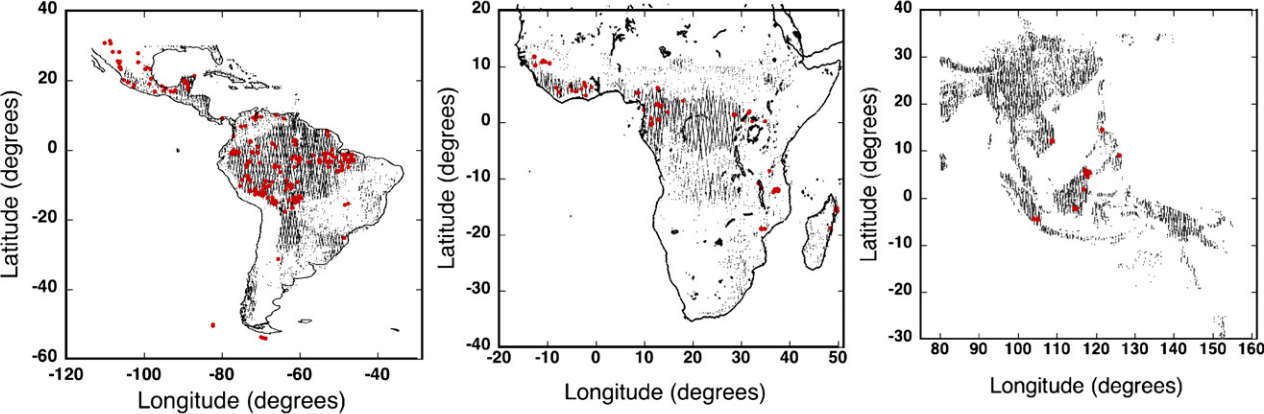
\includegraphics[width=10cm]{figs/carbon/data-saatchi.png}
\caption{\textbf{Field plots used in Saatchi et al. 2011}}
\end{figure}

\begin{itemize}
\item Some countries might be absent from the final map (eg. New Caledonia for Saatchi, WHRC-Baccini and Avitabile's maps).
\item Global models might not be accurate for countries with no field data for calibration.
\item High discrepancies between maps.
\item Resolutions might be coarse: >= 500 m.
\end{itemize}
\end{frame}

\begin{frame}[label={sec:orga816545}]{GEDI derived AGB map}
\begin{columns}
\begin{column}{0.5\columnwidth}
\begin{center}
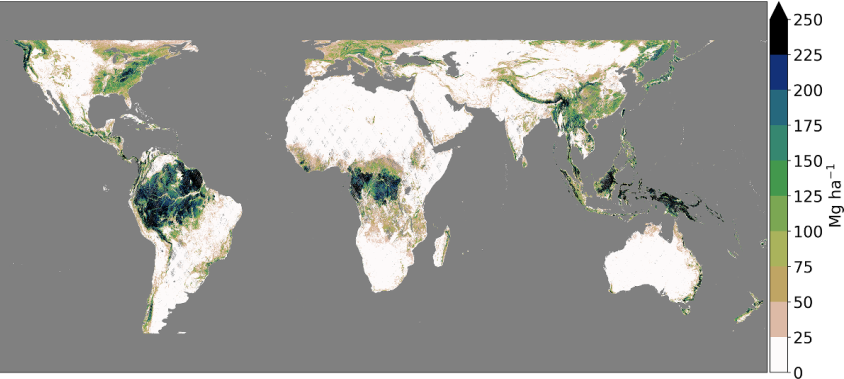
\includegraphics[width=6cm]{figs/carbon/AGB_GEDI.png}
\end{center}
\end{column}

\begin{column}{0.5\columnwidth}
\begin{center}
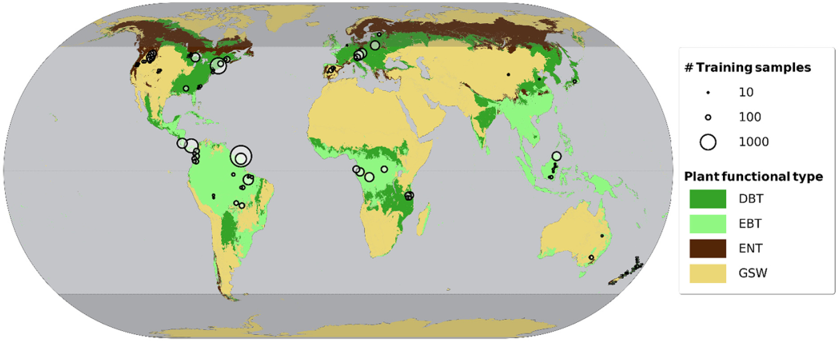
\includegraphics[width=6cm]{figs/carbon/training-data-GEDI.png}
\end{center}
\end{column}
\end{columns}

\begin{block}{}
\begin{itemize}
\item No extrapolation using satellite images and SRTM.
\item GEDI footprints are aggregated within 1 km grid cells.
\item Low resolution: 1 km, location uncertainty of about 25 m.
\item Same problem as for other data-sets: no field data from Melanesia for calibration.
\end{itemize}
\end{block}
\end{frame}

\subsection{National maps}
\label{sec:org516d8e1}

\begin{frame}[label={sec:org05ee776}]{National maps}
\begin{itemize}
\item There is room to improve forest carbon stock maps at the national scale.

\item MELANOBS objectives:
\begin{itemize}
\item Which forest carbon data is available at the national scale?
\item Derive up to date forest carbon stock maps for participating countries.
\end{itemize}
\end{itemize}
\end{frame}

\begin{frame}[label={sec:org28ab2ad}]{In New-Caledonia}
\begin{center}
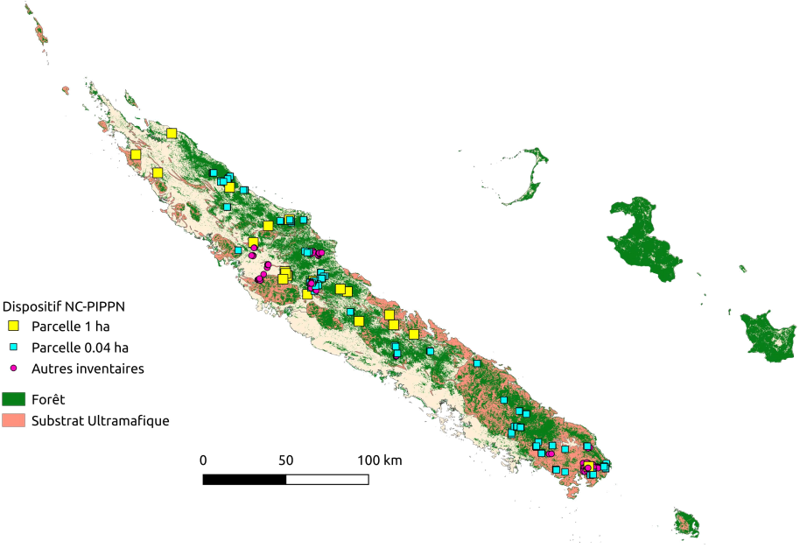
\includegraphics[width=7cm]{figs/carbon/ncpippn-plots.png}
\end{center}

\begin{itemize}
\item No existing national forest carbon stock map.
\item NC-PIPPN forest inventory network + MELANOBS network of 1ha permanent forest plots.
\item LiDAR data.
\item Good cover by GEDI.
\end{itemize}
\end{frame}

\section{Biodiversity maps}
\label{sec:org2ee4f9a}

\subsection{Global biodiversity maps}
\label{sec:orge843bc6}

\begin{frame}[label={sec:orge0d3016}]{Global biodiversity maps}
\begin{center}
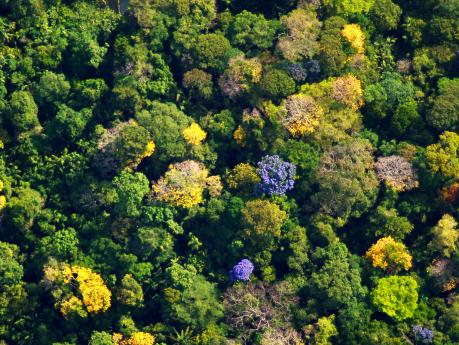
\includegraphics[width=5cm]{figs/aerial-bci.jpg}
\end{center}

\begin{itemize}
\item As a first approximation of biodiversity in forests, we can focus on tree diversity.
\item One objective would be to obtain tree community maps (\(\beta\) diversity).
\item More detailed forest typology than dichotomic dry/moist forests or low-elevation/high-elevation forests.
\item Global maps often represent species richness (\(\alpha\)-diversity). A few examples below.
\end{itemize}
\end{frame}

\begin{frame}[label={sec:orga56e64c}]{Global biodiversity maps}
\begin{center}
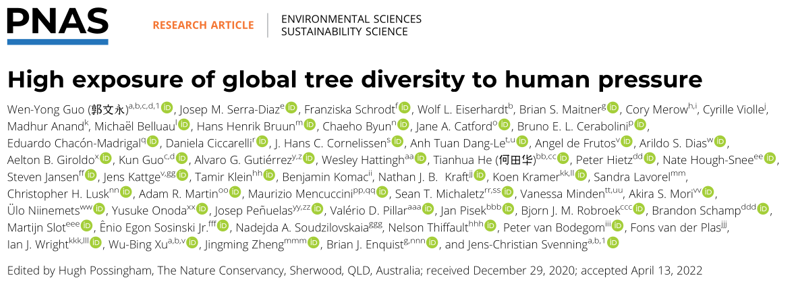
\includegraphics[width=10cm]{figs/biodiv/Guo2022-title.png}
\end{center}

\begin{itemize}
\item SDM for 46,752 tree species from GBIF, BIEN, DRYFLOR, RAINBIO, and ALA datasets.
\item They considered taxonomic, phylogenetic, and functional diversity but disregarded \(\beta\)-diversity.
\end{itemize}
\end{frame}

\begin{frame}[label={sec:orga91c7e6}]{Global biodiversity maps}
\begin{columns}
\begin{column}{0.5\columnwidth}
\begin{center}
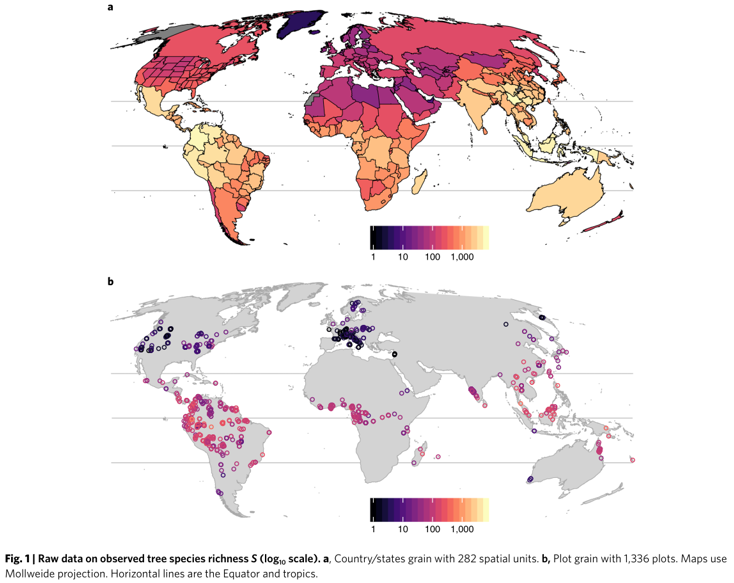
\includegraphics[width=6cm]{figs/biodiv/Keil2019-figure.png}
\end{center}
\end{column}

\begin{column}{0.5\columnwidth}
\begin{center}
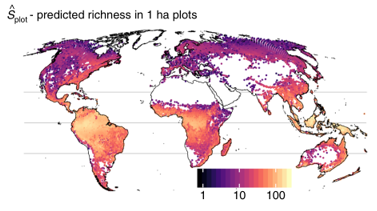
\includegraphics[width=5cm]{figs/biodiv/Keil2019-figure-2.png}
\end{center}

\textbf{Keil \& Chase.} (2019). Global patterns and drivers of tree diversity integrated across a continuum of spatial grains. \emph{Nature Ecology \& Evolution}.
\end{column}
\end{columns}
\end{frame}

\begin{frame}[label={sec:orgba98062}]{Continental biodiversity maps}
\begin{center}
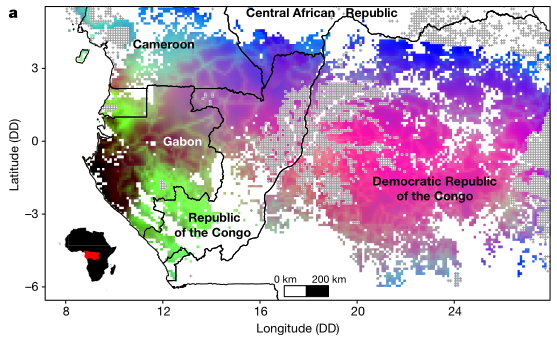
\includegraphics[width=8cm]{figs/biodiv/Rejou-Mechain2021.png}
\end{center}

\textbf{Réjou-Méchain et al.} (2021). Unveiling African rainforest composition and vulnerability to global change. \emph{Nature}.
\end{frame}

\begin{frame}[label={sec:org483f2fe}]{Continental biodiversity maps}
\begin{center}
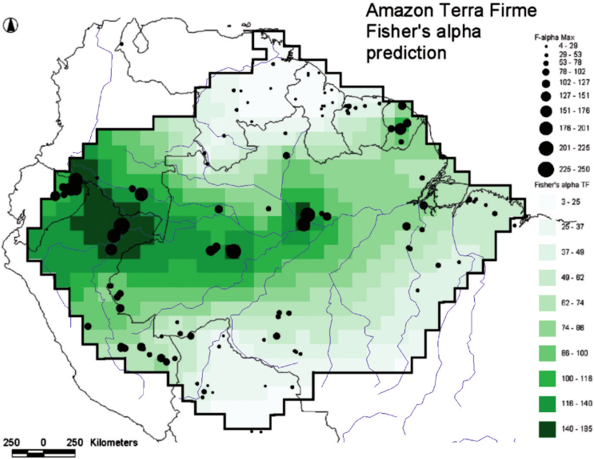
\includegraphics[width=6cm]{figs/biodiv/terSteege2003-figure.png}
\end{center}

\textbf{ter Steege et al.} (2003). A spatial model of tree \(\alpha\)-diversity and tree density for the Amazon. \emph{Biodiversity and Conservation}.
\end{frame}

\subsection{Global biodiversity data-sets}
\label{sec:org1a5ab45}

\begin{frame}[label={sec:org7aa7aa3}]{Global or continental tree data-sets}
\begin{itemize}
\item GBIF: Global Biodiversity Information Facility.
\item BIEN: Botanical Information and Ecology Network.
\item DRYFLOR: Latin American Seasonally Dry Tropical Forest Floristic Network.
\item RAINBIO: mega-database of tropical African vascular plants distributions.
\end{itemize}
\end{frame}

\subsection{National data-sets}
\label{sec:orgb396399}

\begin{frame}[label={sec:org11888a5}]{National data-sets}
\begin{itemize}
\item No global or continental tree community maps that could be used at national scales.
\item But there are global datasets (GBIF, BIEN) that could be used at national scales.
\item MELANOBS objectives:
\begin{itemize}
\item Which tree diversity data is available for each country?
\item Derive first tree community maps for participating countries.
\end{itemize}
\end{itemize}
\end{frame}

\begin{frame}[label={sec:org1e923e1}]{Tree data in New-Caledonia}
\begin{itemize}
\item NOU herbarium data.
\item NC-PIPPN forest plot network with floristic data.
\item Endemia (Red List Authority) data.
\end{itemize}
\end{frame}

\begin{frame}[label={sec:orgf9561b6}]{Mapping tree communities in New Caledonia}
\begin{center}
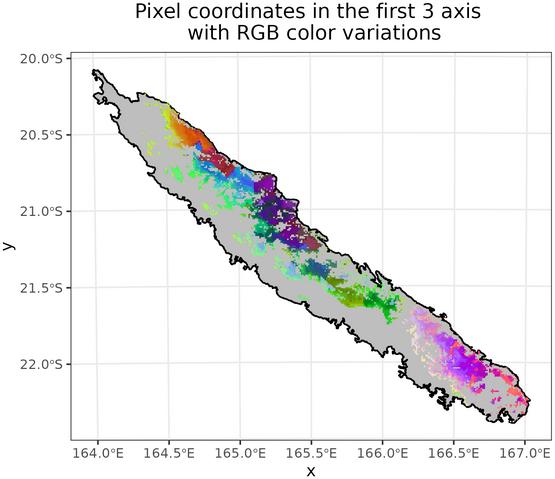
\includegraphics[width=6cm]{figs/biodiv/jSDM-NC.png}
\end{center}

\begin{itemize}
\item Use of joint species distribution models for 878 species and 554 sites.
\item JSDMs: account for species co-occurrence.
\item Predicting species probability of presence for each 1km pixel.
\item Clustering species to obtain tree communities.
\end{itemize}
\end{frame}

\section{Conclusion}
\label{sec:org3b8bc61}

\subsection{Summary}
\label{sec:orgffba79e}

\begin{frame}[label={sec:orge9e2e03}]{Summary}
\begin{itemize}
\item Melanesia is often absent from global forest cover change, carbon, or biodiversity maps.
\item For carbon and biodiversity, global maps are not derived using data from Melanesia (or only a few). They do not have a high accuracy if used at the national scale.
\item \textbf{Objectives}: deriving accurate maps of forest cover change, carbon stocks, and tree communities based on field data from each participating country.
\end{itemize}
\end{frame}

\subsection{Perspectives}
\label{sec:org3bdc486}

\begin{frame}[label={sec:org8b1a252}]{Perspectives}
Several perspectives for forest monitoring and conservation planning:
\begin{itemize}
\item How current deforestation impact carbon emissions and biodiversity loss?
\item Identifying areas of high conservation values with regards to carbon and biodiversity.
\item Anticipating impact on carbon and biodiversity of various deforestation scenarios.
\item Carbon and biodiversity credits associated with avoided deforestation.
\end{itemize}
\end{frame}

% %%%%%%%%%%%%%%%%%%%%%%%%%%%%%%%%%%%%%%%%%%%%%%%%%%%%%%%%%%

{
  % Use background image
  \usebackgroundtemplate{%
    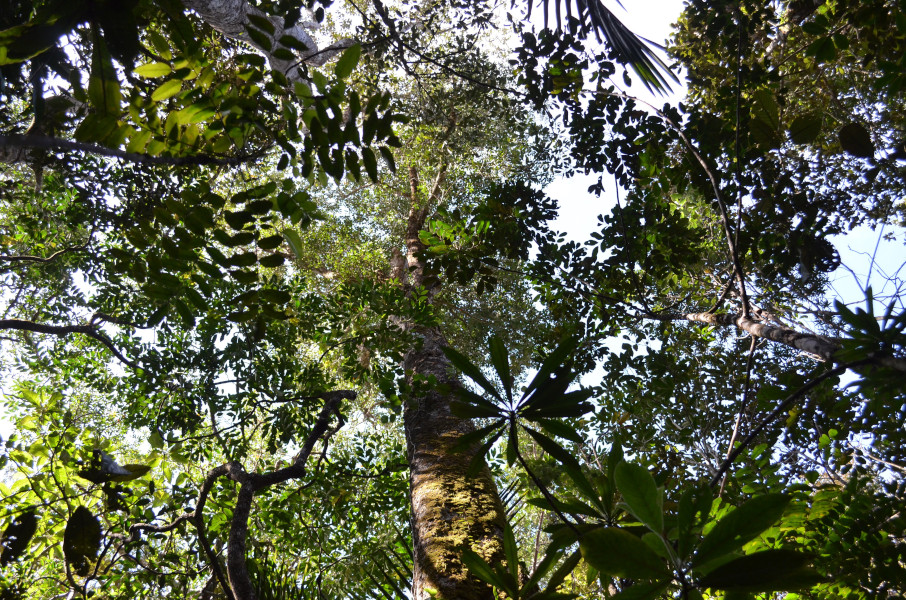
\includegraphics[keepaspectratio=true, height=\paperheight]{figs/Canopy-NC}
  }
  \setbeamertemplate{navigation symbols}{}
  % Remove shadow from block
  \setbeamertemplate{blocks}[rounded][shadow=false]
  \begin{frame}[plain]
  	\vspace*{\stretch{100}} 
    \begin{block}{}
      \begin{center}
        \ldots~Thank you for attention~\ldots \\
        \url{https://ecology.ghislainv.fr/presentations} \\
        
\includegraphics[width=0.6\textwidth]{figs/partners_logos}
      \end{center}
    \end{block}
  \end{frame}
}
\end{document}
